\documentclass{article}
\usepackage{amsmath,amssymb,amsfonts,latexsym}
\usepackage{graphicx}
\usepackage{times}
\usepackage{a4wide}
\usepackage{inputenc}
\usepackage{tikz}
\usepackage{multido}

\usepackage{pgf,tikz,pgfplots}
\pgfplotsset{compat=1.11}

\parindent=0mm
\parskip=2mm

\usepackage[natbib=true,backend=biber,sorting=nyt,style=apa]{biblatex}
\renewcommand*{\bibfont}{\fontsize{10}{12}\selectfont}

\addbibresource{sangwin.bib}

\newtheorem{example}{Example}
\newtheorem{theorem}{Theorem}

\newcommand{\href}[2]{#2}

%\title{Many proofs of the same result: the sum of any number of successive odd numbers beginning from unity}
\title{Proof examples for CJ studies on Rigour and Insight}
\author{Chris Sangwin\footnote{School of Mathematics, University of Edinburgh, Edinburgh, EH9 3FD.  {\tt C.J.Sangwin@ed.ac.uk}}}
\date{}

\begin{document}
	
\maketitle

This document contains many proofs of the following theorem.
\begin{theorem}\label{thm}
  %The sum of any number of successive odd numbers, beginning from unity, is the square of half the even number which follows the last odd number.
  The sum of the first \(n\) odd integers, starting from one, is \(n^2\).
\end{theorem}
Expressed in algebraic notation, this theorem becomes
\begin{equation}\label{eq:thm}
1+3+5+7+\cdots+(2n-1)=\sum_{k=1}^n (2k-1) = n^2.
\end{equation}

The proofs below are a selection from, and adaptation of, those in \autocite{2023-Sum-Odd-Num}.

Participants were not shown the name of the proof or provenance (where known) during the experiment.

\printbibliography{}

\newpage

1. Experimental evidence

From the following
\[ 1 = 1 = 1^2 \]
\[ 1+3 = 4 = 2^2 \]
\[ 1+3+5 = 9 = 3^2 \]
\[ 1+3+5+7 = 16 = 4^2 \]
\[ 1+3+5+7+9 = 25 = 5^2 \]
\[ 1+3+5+7+9+11 = 36 = 6^2 \]
\[ \vdots\]
We clearly see the following pattern holds
\[ 1+3+5+7+\cdots+(2n-1) = n^2.\]


%%%%%%%%%%%%%%%%%%%%%%%%%%%%%%%%%%%%%%%%%%%%%%%%
2. Pictorial I.

\begin{center}
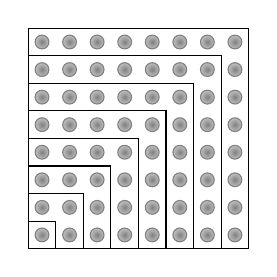
\begin{tikzpicture}[scale=0.35]
\multido{\i=1+1}{8}{%
\draw [draw=black] (0,0) rectangle (\i,\i);
}
\multido{\nx=0.5+1.0}{8}{%
\multido{\ny=0.5+1.0}{8}{%
\shade[inner color=gray,outer color=lightgray] (\nx,\ny) circle (.25);
\draw [gray] (\nx,\ny) circle (.25);
%\draw [gray,fill=lightgray] (\nx,\ny) circle (.25);
}
}
\end{tikzpicture}
\end{center}
\[ 1+3+5+7+\cdots+(2n-1) = n^2.\]

\newpage
%%%%%%%%%%%%%%%%%%%%%%%%%%%%%%%%%%%%%%%%%%%%%%%%
3. Pictorial II.

\begin{center}
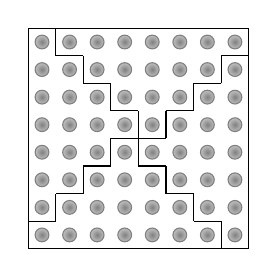
\begin{tikzpicture}[scale=0.35]
\draw [draw=black] (0,0) rectangle (8,8);
\multido{\nx=0.5+1.0}{8}{%
\multido{\ny=0.5+1.0}{8}{%
\shade[inner color=gray,outer color=lightgray] (\nx,\ny) circle (.25);
\draw [gray] (\nx,\ny) circle (.25);
%\draw [gray,fill=lightgray] (\nx,\ny) circle (.25);
}
}
\multido{\i=0+1}{4}{%
\draw (\i,\i+1) -- (\i+1,\i+1);
\draw (\i,\i) -- (\i,\i+1);
%
\draw (\i+1,7-\i) -- (\i+2,7-\i);
\draw (\i+1,8-\i) -- (\i+1,7-\i);
%
\draw (\i+4,3-\i) -- (\i+5,3-\i);
\draw (\i+4,4-\i) -- (\i+4,3-\i);
%
\draw (\i+4,\i+4) -- (\i+5,\i+4);
\draw (\i+5,4+\i) -- (\i+5,5+\i);
}
\end{tikzpicture}
\end{center}
\[ 1+3+5+7+\cdots+(2n-1) = \frac{1}{4}(2n)^2 = n^2.\]


%%%%%%%%%%%%%%%%%%%%%%%%%%%%%%%%%%%%%%%%%%%%%%%%

 4. Arithmetic Progression

\[
1+3+5+7+\cdots+(2n-1)
\]
is an arithmetic progression with difference \(2\) and \(n\) terms. The first term \(a_1=1\), and the last term \(a_n=2n-1\), and the sum of an AP is \( \frac{n}{2}(a_1+a_n)\), which in this case is \(\frac{n}{2}(1+2n-1)=n^2\).

%%%%%%%%%%%%%%%%%%%%%%%%%%%%%%%%%%%%%%%%%%%%%%%%

5. Reversed list

Write the terms twice, with the second list reversed.
\[
\begin{array}{cccccccccc}
1    & + & 3    & + & 5    & + \cdots + & 2n-3 & + & 2n-1 \\
2n-1 & + & 2n-3 & + & 2n-5 & + \cdots + &    3 & + & 1
\end{array}
\]
Each column has total \(2n\) and there are \(n\) columns.  So the total is \(2n^2\) proving \(\sum_{k=1}^n (2k-1) = n^2\).
		
%%%%%%%%%%%%%%%%%%%%%%%%%%%%%%%%%%%%%%%%%%%%%%%%

6. Telescope
		
Notice that \( 2k-1 = k^2 - (k-1)^2\), so that adding up we have
\[ \sum_{k=1}^n (2k-1) = \sum_{k=1}^n k^2 - (k-1)^2\]
However in
\[ \sum_{k=1}^n k^2 - (k-1)^2 = (1^2-0^2)+(2^2-1^2)+(3^2-2^2)+\]
\[\cdots+(n^2-(n-1)^2)\]
all terms cancel except two, one from the first term and one from the last, i.e. \(-0^2+n^2\), leaving \(n^2\).

%%%%%%%%%%%%%%%%%%%%%%%%%%%%%%%%%%%%%%%%%%%%%%%%

7. Backwards reasoning
		
The Fundamental Theorem of Finite Differences says that \(S_n = \sum_{k=1}^n a_k\) if and only if \(a_n = S_{n}-S_{n-1}\).

Consider \(S_n=n^2\) then \[S_n-S_{n-1}=n^2-(n-1)^2=2n-1.\]
Hence  \(\sum_{k=1}^n (2k-1) = n^2\).


%%%%%%%%%%%%%%%%%%%%%%%%%%%%%%%%%%%%%%%%%%%%%%%%

8. Rearranging I
		
We use the standard results \(\sum_{k=1}^n k = \frac{n(n+1)}{2}\) and \(\sum_{k=1}^n 1 = n\) and rearrange
\[ \sum_{k=1}^n (2k-1) = 2\sum_{k=1}^n k - \sum_{k=1}^n 1 = 2\frac{n(n+1)}{2}-n = n^2.\]

%%%%%%%%%%%%%%%%%%%%%%%%%%%%%%%%%%%%%%%%%%%%%%%%
\newpage
9. Rearranging II
	
		
We use the standard result \(\sum_{k=1}^n k = \frac{n(n+1)}{2}\) and rearrange
\[ \sum_{k=1}^n \underbrace{2k-1}_{\mbox{odd}} \]
\[=	(\underbrace{1+2+3+\cdots+2n}_{\mbox{all}}) - (\underbrace{2+4+6+\cdots +2n}_{\mbox{even}})\]
\[= (1+2+3+\cdots+2n) - 2(1+2+3+\cdots +n)\]
Hence
\[ \sum_{k=1}^n (2k-1) = \sum_{k=1}^{2n} k -  2\sum_{k=1}^{n} k\]
\[ = \frac{2n(2n+1)}{2} - 2\frac{n(n+1)}{2} = n^2.\]

%%%%%%%%%%%%%%%%%%%%%%%%%%%%%%%%%%%%%%%%%%%%%%%%

10. Induction
		
Let \(P(n)\) be the statement \(\sum_{k=1}^n (2k-1) = n^2\).
	
Since \(\sum_{k=1}^1 (2k-1) = 1 = 1^2\) we see \(P(1)\) is true.
		
Assume \(P(n)\) is true then
\[ \sum_{k=1}^{n+1} (2k-1) = \sum_{k=1}^n (2k-1) + (2(n+1)-1) \]
\[= n^2 + 2n +1 = (n+1)^2.\]
Hence \(P(n+1)\) is true.
		
Since \(P(1)\) is true and \(P(n+1)\) follows from \(P(n)\) we conclude that \(P(n)\) is true for all \(n\) by the principle of mathematical induction.

%%%%%%%%%%%%%%%%%%%%%%%%%%%%%%%%%%%%%%%%%%%%%%%%

11. Contradiction
		
To prove \(\forall\, n\in\mathbb{N}: \sum_{k=1}^n (2k-1) = n^2\),
assume, for a contradiction, that \(\exists\, n\in\mathbb{N}: \sum_{k=1}^n (2k-1) \neq n^2\).
Let \(n^*\) be the smallest such example.  Note, \(n^*>1\) since \((2\times 1)-1 = 1^2\).
		
If \(\sum_{k=1}^{n^*} (2k-1) > {n^*}^2\) then
\[ \sum_{k=1}^{n^*} (2k-1) = 2n^*-1 + \sum_{k=1}^{n^*-1} (2k-1) > {n^*}^2\]
and so
\[ \sum_{k=1}^{n^*-1} (2k-1) > {n^*}^2 - 2n^*+1 = (n^*-1)^2.\]
This proves \(\sum_{k=1}^{n^*-1} (2k-1) \neq (n^*-1)^2\), which contradicts the minimality of \(n^*\).  The case \(\sum_{k=1}^{n^*} (2k-1) < {n^*}^2\) leads to an identical contradiction.
		
%%%%%%%%%%%%%%%%%%%%%%%%%%%%%%%%%%%%%%%%%%%%%%%%
\newpage

12. Linear system
		
Since the sum is always an integer and
\[S_n=\sum_{k=1}^{n} (2k-1) \leq n(2n-1)\]
the growth of \(S_n\) is quadratic in \(n\).  We therefore assume
\[ \sum_{k=1}^{n} (2k-1) = an^2 + bn +c\quad \forall\, n\in \mathbb{N}.\]
Since this formula holds for all \(n\) it must hold for \(n=1,2,3\).  Hence
\[
\begin{array}{lcll}
1    & = & a+b+c,   & (n=1)    \\
1+3  & = & 4a+2b+c, & (n=2)  \\
1+3+5& = & 9a+3b+c, & (n=3)\\
\end{array}
\]
This is a linear system in \(a,b,c\) which we set up as
\[ \left( \begin{array}{ccc} 1 & 1 & 1 \\ 4 & 2 & 1 \\ 9 & 3 & 1 \end{array} \right) \left(\begin{array}{c} a \\ b \\ c \end{array}\right) = \left(\begin{array}{c} 1 \\ 4 \\ 9\end{array}\right).\]
The matrix clearly has non-zero determinant, so the system has a unique solution.
This solution is (exercise to check) \(a=1\), \(b=c=0\).  Hence \(\sum_{k=1}^n (2k-1) = n^2\).

%%%%%%%%%%%%%%%%%%%%%%%%%%%%%%%%%%%%%%%%%%%%%%%%

13 Undetermined coefficients

Assume
\[1+3+5+7+\cdots + (2n-1) \]
\[= A+Bn+Cn^2+Dn^3+En^4+\cdots .\]
Then
\[  1+3+5+7+\cdots + (2n-1)+(2(n+1)-1) \]
\[ = A+B(n+1)+C(n+1)^2+D(n+1)^3+E(n+1)^4+\cdots\]
Subtracting
\[ 2n+1=B+C(2n+1)+D(3n^2+3n+1)\]
\[ +E(4n^3+6n^2+4n+1) + \cdots\]
Equating powers of \(n^2,n^3,\cdots\) on both sides we see \(D=E=...=0\).
\[ 2n+1=B+C(2n+1).\]
Hence \(B=0\) and \(C=1\), from which \(A=0\) and so \(\sum_{k=1}^n (2k-1) = n^2\).

%%%%%%%%%%%%%%%%%%%%%%%%%%%%%%%%%%%%%%%%%%%%%%%%

14 Induction  (b)

Consider the conjecture \(\sum_{k=1}^n (2k-1) = n^2\).
First note \(\sum_{k=1}^1 (2k-1) = 1 = 1^2\).
Now,
\[ \sum_{k=1}^{n+1} (2k-1) = \sum_{k=1}^n (2k-1) + (2(n+1)-1) = n^2 + 2n +1 = (n+1)^2.\]
Hence \(\sum_{k=1}^n (2k-1) = n^2\) by induction.

%%%%%%%%%%%%%%%%%%%%%%%%%%%%%%%%%%%%%%%%%%%%%%%%
\newpage
15 Pictorial II (b)

In the picture below, each stepped triangle has
\(1+3+5+\cdots+(2n-1)\) dots.
\begin{center}
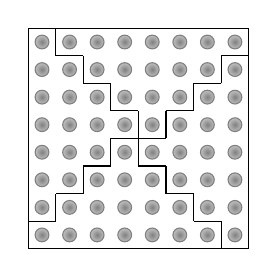
\begin{tikzpicture}[scale=0.35]
\draw [draw=black] (0,0) rectangle (8,8);
\multido{\nx=0.5+1.0}{8}{%
\multido{\ny=0.5+1.0}{8}{%
\shade[inner color=gray,outer color=lightgray] (\nx,\ny) circle (.25);
\draw [gray] (\nx,\ny) circle (.25);
%\draw [gray,fill=lightgray] (\nx,\ny) circle (.25);
}
}
\multido{\i=0+1}{4}{%
\draw (\i,\i+1) -- (\i+1,\i+1);
\draw (\i,\i) -- (\i,\i+1);
%
\draw (\i+1,7-\i) -- (\i+2,7-\i);
\draw (\i+1,8-\i) -- (\i+1,7-\i);
%
\draw (\i+4,3-\i) -- (\i+5,3-\i);
\draw (\i+4,4-\i) -- (\i+4,3-\i);
%
\draw (\i+4,\i+4) -- (\i+5,\i+4);
\draw (\i+5,4+\i) -- (\i+5,5+\i);
}
\end{tikzpicture}
\end{center}
Four copies of this triangle can be fitted together to give a square where the side length is \\ \((2n-1)+1\) so the number of dots is \((2n)^2\).

Hence
\[ 1+3+5+7+\cdots+(2n-1) = \frac{1}{4}(2n)^2 = n^2.\]
	
%\begin{center}
%\begin{minipage}{7.5cm}
%In the picture below, each stepped triangle has
%\(1+3+5+\cdots+(2n-1)\) dots.
%\end{minipage}
%
%\begin{tikzpicture}[scale=0.35]
%\draw [draw=black] (0,0) rectangle (8,8);
%\multido{\nx=0.5+1.0}{8}{%
%\multido{\ny=0.5+1.0}{8}{%
%\shade[inner color=gray,outer color=lightgray] (\nx,\ny) circle (.25);
%\draw [gray] (\nx,\ny) circle (.25);
%%\draw [gray,fill=lightgray] (\nx,\ny) circle (.25);
%}
%}
%\multido{\i=0+1}{4}{%
%\draw (\i,\i+1) -- (\i+1,\i+1);
%\draw (\i,\i) -- (\i,\i+1);
%%
%\draw (\i+1,7-\i) -- (\i+2,7-\i);
%\draw (\i+1,8-\i) -- (\i+1,7-\i);
%%
%\draw (\i+4,3-\i) -- (\i+5,3-\i);
%\draw (\i+4,4-\i) -- (\i+4,3-\i);
%%
%\draw (\i+4,\i+4) -- (\i+5,\i+4);
%\draw (\i+5,4+\i) -- (\i+5,5+\i);
%}
%\end{tikzpicture}
%
%\begin{minipage}{7.5cm}
%Four copies of this triangle can be fitted together to give a square where the side length is \\ \((2n-1)+1\) so the number of dots is \((2n)^2\).
%
%Hence
%\[ 1+3+5+7+\cdots+(2n-1) = \frac{1}{4}(2n)^2 = n^2.\]
%\end{minipage}
%\end{center}

\end{document}

